%% LyX 2.1.4 created this file.  For more info, see http://www.lyx.org/.
%% Do not edit unless you really know what you are doing.
\documentclass[11pt]{article}
\usepackage[latin9]{inputenc}
\usepackage{geometry}
\geometry{verbose}
\usepackage{fancyhdr}
\pagestyle{fancy}
\usepackage{amsmath}
\usepackage{amssymb}
\usepackage{graphicx}
\usepackage{esint}

\makeatletter
%%%%%%%%%%%%%%%%%%%%%%%%%%%%%% User specified LaTeX commands.
\usepackage[margin=0.75in]{geometry} % see geometry.pdf on how to lay out the page. There's lots.
\usepackage{graphicx}
\usepackage{cleveref}
\usepackage{amsmath}
\usepackage{multirow}
\usepackage{listings}
\usepackage{color}
\usepackage{CJK}
\definecolor{mygreen}{RGB}{28,172,0}
\definecolor{mylilas}{RGB}{170,55,241}

\usepackage[latin9]{inputenc}
\geometry{verbose}


\makeatletter
\@ifundefined{date}{}{\date{}}
\makeatother

%Fancy-header package to modify header/page numbering 
\usepackage{fancyhdr}
\pagestyle{fancy}
\lhead{\textbf{Ge/ESE 118}} %name of the course
\chead{\textbf{}} %topic of the homework set
\rhead{\textbf{Solution 2}} %number of the homework set
\lfoot{}
\cfoot{}
\rfoot{\thepage}


% Matlab script
\lstset{language=Matlab,%
      %basicstyle=\color{red},
  breaklines=true,%
  morekeywords={matlab2tikz},
  keywordstyle=\color{blue},%
  morekeywords=[2]{1}, keywordstyle=[2]{\color{black}},
  identifierstyle=\color{black},%}
  stringstyle=\color{mylilas},
  commentstyle=\color{mygreen},%
  showstringspaces=false,%without this there will be a symbol in the places where there is a space
  numbers=left,%
  numberstyle={\tiny \color{black}},% size of the numbers
  numbersep=9pt, % this defines how far the numbers are from the text
  emph=[1]{for,end,break},emphstyle=[1]\color{red}, %some words to emphasise
                                                      %emph=[2]{word1,word2}, emphstyle=[2]{style},    
}

\makeatother

\begin{document}

\subsection*{Problem 1 (graded by Yiran) 40 points}


\subsubsection*{(a) - 5 points}

The misfit function 
\begin{eqnarray*}
F(\boldsymbol{m}) & = & \sum_{i}\frac{(d_{i}-g_{i}(\boldsymbol{m}))^{2}}{2\sigma_{d}^{2}}
\end{eqnarray*}


Then, the posterior PDF

\begin{eqnarray*}
P(\boldsymbol{m}|\boldsymbol{d})\propto P(\boldsymbol{d}|\boldsymbol{m})\propto\exp\left(-F(\boldsymbol{m})\right)\approx\exp\left(-F(\boldsymbol{m}_{0})-\frac{\partial F}{\partial\boldsymbol{m}}^{T}(\boldsymbol{m}-\boldsymbol{m}_{0})-\frac{1}{2}(\boldsymbol{m}-\boldsymbol{m}_{0})^{T}\frac{\partial^{2}F}{\partial\boldsymbol{m}\partial\boldsymbol{m}}(\boldsymbol{m}-\boldsymbol{m}_{0})\right)
\end{eqnarray*}
 has the form of a multivariate Gaussian distribution, and the covariance
matrix is 
\begin{eqnarray*}
cov(\boldsymbol{m})=\left(\frac{\partial^{2}F}{\partial\boldsymbol{m}\partial\boldsymbol{m}}|_{\boldsymbol{m}=\boldsymbol{m}_{0}}\right)^{-1}=\boldsymbol{H}^{-1}
\end{eqnarray*}
Note we want to know covariance matrix when $m_{0}$ is the least
squares solution. 

Using HW2's convention, define 
\begin{eqnarray*}
\hat{G}_{i,k}=\frac{\partial g_{i}}{\partial m_{k}}
\end{eqnarray*}


Then

\begin{eqnarray*}
H\approx\frac{\hat{G}^{T}\hat{G}}{\sigma_{d}^{2}}
\end{eqnarray*}


In HW2, we didn't include the data error in the hessian. So we need
to modify it by dividing $\sigma_{d}^{2}$ when calculate the model
covariance matrix. 

(See MATLAB code) The output model covariance matrix is:
\begin{verbatim}
    0.0101   -0.0123    0.0095    0.0548    
   -0.0123    0.0198   -0.0156   -0.0853     
    0.0095   -0.0156    0.0237    0.1034     
    0.0548   -0.0853    0.1034    0.4985
\end{verbatim}

\subsubsection*{(b)- 5 points}

The covariance matrix calculated here will be similar to the Monte
Carlo simulation in HW2.

Diagonal element shows the variance of each parameter. The square
root of the diagonal elements gives the standard deviations: $\sigma_{x_{s}}=0.1006$,
$\sigma_{y_{s}}=0.1405$, $\sigma_{z_{s}}=0.1538$, $\sigma_{P}=0.7060$.
The number is very close to that estimated before: $\sigma_{x_{s}}=0.099670,\sigma_{y_{s}}=0.137469,\sigma_{z_{s}}=0.149719,\sigma_{P}=0.691071$.

The off diagonal shows the covariance between parameters. We can scale
the covariance matrix to correlation matrix ($\rho_{xy}=\frac{\sigma_{xy}}{\sigma_{x}\sigma_{y}}$).
The correlation matrix is:
\begin{verbatim}
    1.0000   -0.8685    0.6127    0.7721    
   -0.8685    1.0000   -0.7200   -0.8598     
    0.6127   -0.7200    1.0000    0.9520     
    0.7721   -0.8598    0.9520    1.0000
\end{verbatim}
we see that there are strong trade-offs between mode parameters. The
strong negative correlation between $x_{s}$ and $y_{s}$, for example,
is also shown in the plot in HW2.


\subsubsection*{(c)- 5 points}

Now 
\begin{eqnarray*}
F(\boldsymbol{m}) & = & \frac{1}{2\sigma^{2}}(\boldsymbol{d}-\boldsymbol{Gm})^{T}(\boldsymbol{d}-\boldsymbol{Gm})
\end{eqnarray*}
where $\sigma=0.1$, and 
\begin{eqnarray*}
\boldsymbol{G} & = & \left[\begin{array}{cc}
\boldsymbol{1} & \boldsymbol{x}\end{array}\right]\\
\boldsymbol{m} & = & [m1,m2]^{T}
\end{eqnarray*}
The Hessian is 
\begin{eqnarray*}
\boldsymbol{H} & = & \frac{1}{\sigma^{2}}\boldsymbol{G}^{T}\boldsymbol{G}
\end{eqnarray*}
and 
\begin{eqnarray*}
cov(\boldsymbol{m}) & = & \boldsymbol{H}^{-1}
\end{eqnarray*}


(see MATLAB code) The output covariance matrix is:
\begin{verbatim}
   1.0e-03 *
    0.3429   -0.0019    
   -0.0019    0.0004
\end{verbatim}

\subsubsection*{(d)- 5 points}

The model covariance is calculated from the distribution $P(\boldsymbol{m}|\boldsymbol{d})$.
The square root of the eigenvalues and eigenvectors of the model covariance
matrix measure the shape (length and direction of the semiaxes) of
the isocontour of $P(\boldsymbol{m}|\boldsymbol{d}$). The shape of
the isocontour of $P(\boldsymbol{m}|\boldsymbol{d})\propto P(\boldsymbol{d}|\boldsymbol{m})\propto\exp(-F(\boldsymbol{m}))$
is scaled to the isocontour of the error ellipse $F(\boldsymbol{m})$
, which we plotted in HW2.

The eigenvectors of the covariance matrix are:$\left[\begin{array}{cc}
-0.0054 & -1.0000\end{array}\right]$ and $\left[\begin{array}{cc}
-1.0000 & 0.0054\end{array}\right]$, correspond to an angle of $89.7^{o}$ and $179.7^{o}$ measured
clockwise from x axis; the ratio of the length of the semiaxis is
$\sqrt{\lambda_{1}}/\sqrt{\lambda_{2}}=0.0319$. We see that it is
true for the error ellipse as shown below (notice the difference in
the scale of x and y axis).

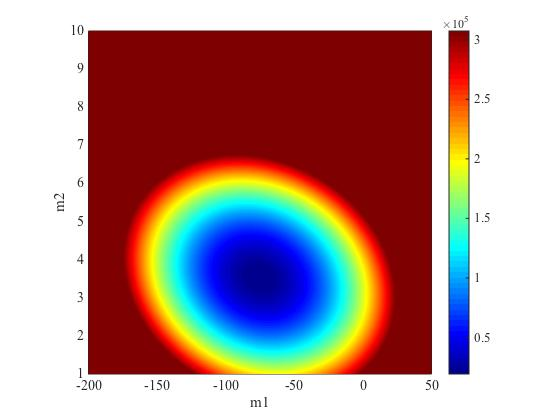
\includegraphics{p1_figures/errorellip}


\subsubsection*{(e)- 5 points}

First calculate the misfit $F(\boldsymbol{m})$ for the full parameter
space.

From Bayesian law and uniform prior,

\begin{eqnarray*}
P(\boldsymbol{m}|\boldsymbol{d}) & \propto & P(\boldsymbol{d}|\boldsymbol{m})\\
 & \propto & \exp(-F(\boldsymbol{m}))\\
\end{eqnarray*}


Normalize the pdf so its integral over the model space equals 1.

\begin{eqnarray*}
P(\boldsymbol{m}|\boldsymbol{d}) & = & \frac{\exp(-F(\boldsymbol{m}))}{\int\exp(F(\boldsymbol{m})d\boldsymbol{m})}
\end{eqnarray*}


that is

\begin{eqnarray*}
P(m_{1},m_{2}|\boldsymbol{d}) & = & \frac{\exp(-F(m_{1},m_{2}))}{\int\int P(m_{1},m_{2}|d)dm_{1}dm_{2}}
\end{eqnarray*}


The marginals are: 
\begin{eqnarray*}
P(m_{1}|d) & = & \int P(m_{1},m_{2}|d)dm_{2}\\
P(m_{2}|d) & = & \int P(m_{1},m_{2}|d)dm_{1}\\
\end{eqnarray*}


We can approximate the integral with rectangle method: $\int f(x)dx=\sum_{i}f(x_{i})\triangle x$.

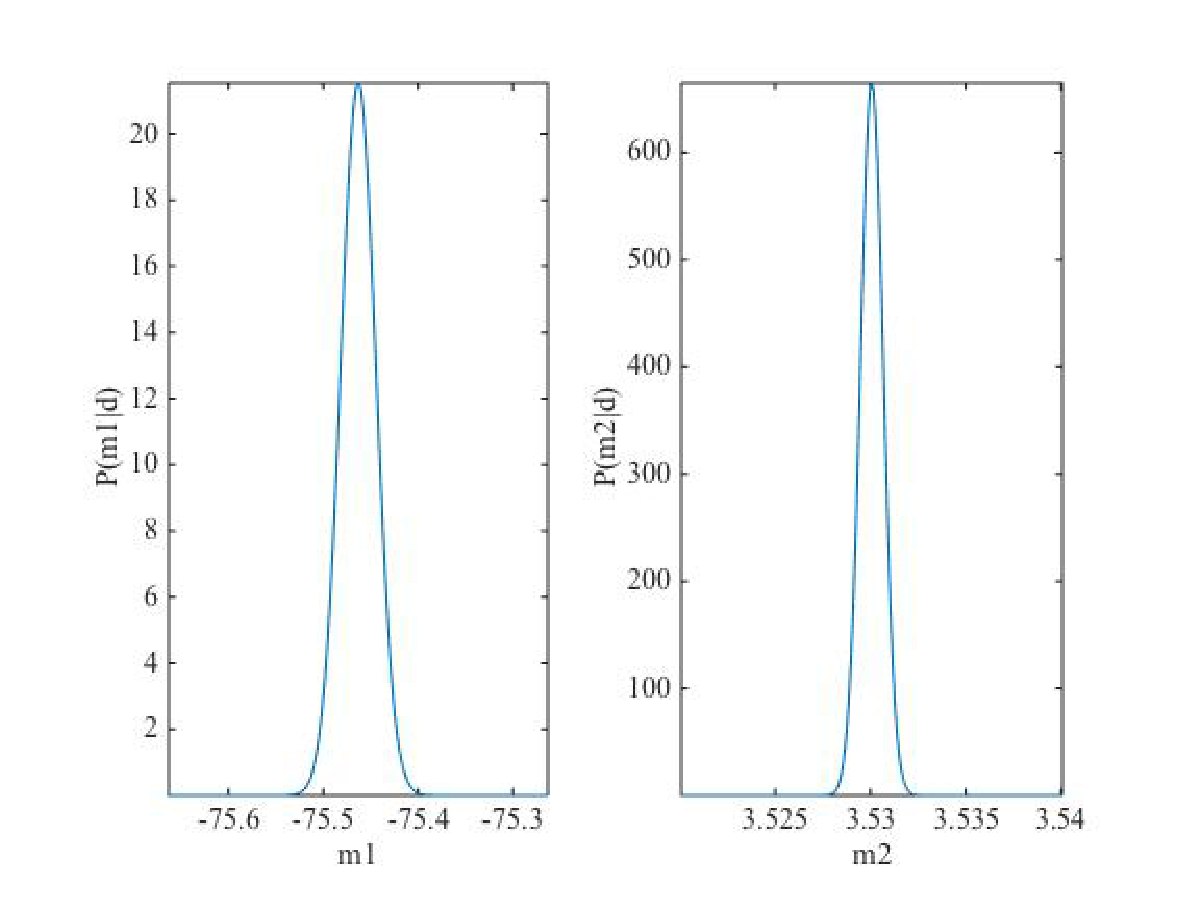
\includegraphics{p1_figures/margin}


\subsubsection*{(f)- 5 points}

By definition

\begin{eqnarray*}
\sigma_{m_{i}}^{2}=E[m_{i}^{2}]-(E[m_{i}])^{2} & = & \int p(m_{i}|d)m_{i}^{2}dm_{i}-\left(\int p(m_{i}|d)m_{i}dm_{i}\right)
\end{eqnarray*}


(see MATLAB code) We get $\sigma_{m1}=0.0185$, $\sigma_{m2}=0.0006$,
which are equal to square root of the diagonal elements of the covariance
matrix calculated in (c).


\subsubsection*{MATLAB code for (a)-(b)}

\tiny
\lstinputlisting{p1/hw2_1.m}
\normalsize


\subsubsection*{MATLAB code for (c)-(f)}

\tiny
\lstinputlisting{p1_2/hw2_2.m}
\normalsize

\clearpage{}
\end{document}
